% -*- coding: utf-8 -*-
% !TeX encoding = UTF-8
% !TeX root = ../report.tex


%% kunne være en ide at inkludere den sort-hvide udgave af det endelige moneca kort, bare så de kan se hvad pokker det egentligt handler om. Sætte det ind i starten som en lille figur.


%%%%%%%%%%%%%%%%%%%%%%%%%%%%%%%%%%%%%%%%%%%%%%%%%%%%%%%%%%%
\chapter{Social netværksanalyse \label{metode_sna}}
%%%%%%%%%%%%%%%%%%%%%%%%%%%%%%%%%%%%%%%%%%%%%%%%%%%%%%%%%%%

I dette speciale tilgår vi arbejdsmarkedet som et netværk af forskellige arbejdsstillinger. I netværket bevæger individer sig mellem forskellige typer af arbejdsstillinger. Det sker når en person går fra at være beskæftiget i en arbejdsstilling til at være beskæftiget i en anden arbejdsstilling.

Arbejdsstillingerne betragtes som noder i et netværk, og personernes bevægelser mellem forskellige arbejdsstillinger bestemmes som forbindelserne i netværket. Det er motiveret teoretisk i afsnit ???? og skal ikke uddybes yderligere her. Formålet med at anskue arbejdsmarkedet som et netværk er at kortlægge beskæftigelsesmønstre på arbejdsmarkedet for at se, hvilke arbejdsstillinger de ledige bevæger sig imellem, og hvilke arbejdsstillinger de ikke bevæger sig imellem. Vi har tidligere beskrevet arbejdssegmenteringsteorier kort, og vi vil her gå i dybden med vores centrale metodiske værktøj, social netværksanalyse, i en specifik udgave, som Toubøl og Larsen har udviklet til analyser af mobilitet. Denne metode har de kaldet Moneca - “\emph{Mobility Network Clustering Algorithm}”.  

%begge disse to afsnit bør nok ikke stå her. Skal skrives sammen når vi er færdige #todo

Dette afsnit uddyber og forklarer de centrale antagelser og beregninger i Toubøl og Larsens to artikler om deres nyopfundne metode, samt opridser fundamentale begreber i netværksanalysen efterhånden som de introduceres i forbindelse med gennemgangen af Moneca. Da der er tale om en ny anvendelse af social netværksanalyse, er der ikke meget andet litteratur at benytte sig af end de to forfatteres to artikler, da vi er de første udover omtalte skabere af metoden, der benytter sig af den. Et delmål for dette speciale er derfor at undersøge, hvad Moneca-algoritmen er i stand til, samt være opmærksom på dens eventuelle begrænsinger og mulige fejlbehæftninger. Det er derfor et delmål for dette speciale at evaluere hvorledes Moneca fungerer i relation til videnskabelige mål for reliabilitet og validitet. Dette vil løbende blive diskuteret i specialet, men først skal algoritmens grundlæggende funktioner beskrives.


%  skriv noget med at begrebet klynge og segment vil blive brugt nogenlunde ens


%%%%%%%%%%%%%%%%%%%%%%%%%%%%%%%%%%%%%%%%%%%%%%%%%%%%%%%%%%%
\subsection{Grundlæggende begreber og datastruktur i social netværksanalyse}
%%%%%%%%%%%%%%%%%%%%%%%%%%%%%%%%%%%%%%%%%%%%%%%%%%%%%%%%%%%

Moneca er en overordnet set en kvantitativ, deskriptiv metode, hvis formål er: 
%
\begin{enumerate} \label{monecaformaal}
  \item at vise tilstedeværelsen, fraværet og styrken af relationer mellem forskellige grundkategorier af interesse.
  \item at benytte et sæt kriterier baseret på centrale mål indenfor social netværksanalyse til at slå disse grundkategorier sammen i større grupper, herfra kaldet \emph{segmenter}. Deraf navnet Moneca: \emph{Mobility Network Clustering Algorithm}.
\end{enumerate}
%
Grundkategorierne bestemmes ud fra det empiriske formål. Toubøl og Larsen har benyttet Moneca til at se på den sociale mobilitet mellem forskellige beskæftigelseskategorier indenfor hele det danske arbejdsmarked. Relationerne defineres som skift fra et arbejde indenfor én beskæftigelseskategori til arbejde indenfor en anden beskæftigelseskategori. Herefter benyttes Moneca-algoritments 2. skridt til at undersøge, hvorledes denne datadrevne inddeling af arbejdsmarkedet i segmenter kan give ny indsigt i klasseinddelingen. 


Det centrale er derfor hvilke grundkategorier, der benyttes, samt hvad der tæller som en relation mellem to grundkategorier. Toubøl og Larsen kommer selv med andre forslag til mulige anvendelser af Moneca, eksempelvis kortlægning af klassemobilitet gennem ægteskaber \parencite[27]{Touboel2013}. Her ville grundkategorierne blive bestemt ud fra en given klasseinddeling af interesse, og relationerne mellem disse klasser defineres som ægteskaber. I netværksterminologi betegnes kategorierne som \emph{noder}, mens relationerne mellem noderne betegnes som \emph{edges}, eller på dansk: forbindelser.%
%
\footnote{Det er ofte en udfordring at oversætte de tekniske termer fra netværksanalyse til dansk. Hvor det ikke har været muligt  at benytte et tilstrækkeligt unikt oversat dansk begreb, har vi derfor beholdt de engelske termer.}%
%
. I vores speciale ligger vi derfor konceptuelt helt lig Toubøl \& Larsen, når vi definerer vores noder som beskæftigelseskategorier, og edges som skift mellem disse kategorier%
%
\footnote{Omend forskellen i populationsdefinition - ledige fremfor alle beskæftigede - har stor betydning for den konkrete operationalisering af begreberne, hvilket vil blive behandlet i de efterfølgende kapitler.}%
%
. Vi har det til fælles, at vi ser på en social mobilitetstabel, der viser skift fra beskæftigelseskategorierne i rækkerne til beskæftigelseskategorierne i kolonnerne. Denne er illustreret i tabel \ref{tab_adjacencyeks} ved hjælp af empirisk data fra vores mobilitetstabel.
%
\begin{table}[H] \centering
\caption{Eksempel på en adjacency matrice}
\label{tab_adjacencyeks}
\resizebox{0.8\textwidth}{!}{%
\begin{tabular}{@{}l|cccc@{}} \toprule
	                & Til: Tandlæge & Til: Folkeskolelærer & Til: Pædagog & Til: Automekaniker \\ \midrule
	Fra: Tandlæge        & 264      & 0               & 0       & 0             \\ 
	Fra: Folkeskolelærer & 0        & 6148            & 288     & 6             \\ 
	Fra: Pædagog         & 0        & 454             & 9308    & 0             \\ 
	Fra: Automekaniker   & 0        & 13              & 13      & 1861          \\ \bottomrule
\end{tabular} }
\end{table}
% 

I netværkstermer kaldes sådan en tabel for en \emph{adjacency matrice}, da den har samme udfald i både rækker og kolonner, og datamatricen derfor er kvadratisk \parencite[55]{Scott2000}. I vores tilfælde skal det tolkes sådan, at rækkeudfaldene er de beskæftigelseskategorier, man kom \emph{fra}, og kolonneudfaldene er de beskæftigelseskategorier man er gået \emph{til}, efter en ledighedsperiode. Det ses at 264 personer på et tidspunkt har skiftet fra tandlæge til tandlæge i løbet af de 14 år, og ikke har skiftet til nogle af de andre tre erhverv. Skift fra samme beskæftigelse til samme beskæftigelse som fra tandlæge til tandlæge, noteres grundet den kvadratiske form langs diagonalen i en adjacency matrice, og denne har derfor en særlig status. Vi har at gøre med en \emph{retningsbestemt}, \emph{vægtet} adjacency matrice, hvilket er den mest komplicerede form for  data i social netværksanalyse \parencite[61]{Scott2000}. Med vægtet skal forstås, at de enkelte celler ikke bare tilkendegiver en binær opdeling i tilstedeværelse eller fravær af en forbindelse, eksempelvis mellem folkeskolelærer og automekaniker, men at den også angiver en værdi for styrken af denne forbindelse. At den er retningsbestemt betyder at matricen ikke er symmetrisk langs diagonalen, da bestemmelsen af retningen sker ud fra hvorvidt man ser på et udfald rækkevis eller kolonnevis. Samt - i en vægtet matrice - kan styrken naturligvis også variere alt efter om man befinder sig over eller under diagonalen. I tilfældet automekaniker ses det, at hvis man i matricens nederste del kigger på Automekaniker, er relationen til tandlæge 0, det vil sige fraværende, mens den til folkeskolelærer og pædagog har en styrke på 13 i begge tilfælde. I selve diagonalen, det  vil sige \emph{den interne mobilitet}, er styrken forventeligt langt højere. Hvis man ser på automekaniker i matricens øverste del, det vil sige kolonnevis, er der et fravær af forbindelse til tandlæge, en styrke på 6 til folkeskolelærerer, og et fravær af forbindelse til pædagoger. Det viser hvad der menes med en retningsbestemt, vægtet adjacency matrice: Styrken i mobiliteten fra automekaniker til folkeskolelærer er på 13, mens den fra pædagog til automekaniker er på 6, altså halvt så kraftig.



%%%%%%%%%%%%%%%%%%%%%%%%%%%%%%%%%%%%%%%%%%%%%%%%%%%%%%%%%%%
\subsection{Relativ risiko og styrken af forbindelser \label{metode_relativrisiko}}
%%%%%%%%%%%%%%%%%%%%%%%%%%%%%%%%%%%%%%%%%%%%%%%%%%%%%%%%%%%

Indtil videre har vi kun talt om styrken af forbindelser som antallet af skift, altså en absolut enhed. Det er imidlertidig ikke særlig retvisende, da styrken af forbindelsen dermed ikke står relativt til størrelsen af den kategori, den udspringer af. I 1996 var der eksempelvis 5.207 tandlæger, mens der var 53.676 beskæftigede pædagoger, altså omtrent ti gange så mange. Et skift fra tandlæge til en anden profession bør derfor vægtes højere end et skift fra pædagog til en anden profession.  Her kommer konceptet relativ risiko ind i billedet, som en ratio mellem to proportioner \parencite[244, 271]{Agresti1997}: 
%
\begin{align} 
\frac{\pi_{A}}{\pi_{B}}
\end{align} 
%
Den relative risiko (RR) fortæller os hvad chancen er for at begivenhed B sker, relativt til begivenhed A. Begivenhed A kender vi. Det er den simultane sandsynlighed for udfald \emph{x} og udfald \emph{y} i de to stokastiske variable \emph{I} og \emph{J} () \parencite[41]{Malchow-Moeller2003}, givet ved sandsynlighedsfunktionen:
%
\begin{align} 
f(i,j) = P(I=i, J=j)
\end{align} 
%
I eksemplet fra tabel \ref{tab_adjacencyeks} er den simultane sandsynlighed for at have skiftet fra folkeskolelærer til pædagog: $\frac{45}{45} = 0,45 = \pi_{A}$. Begivenhed B er til vores formål%
%
\footnote{Indenfor medicinsk forskning vil relativ risiko typisk blive brugt sammen med oddsratio-værdier til at bestemme risici mellem en gruppe patienter tildelt en ny medicin samt en kontrolgruppe. Relativ risiko bruges derfor typisk til at vurdere forskelle mellem to konkrete grupper. Toubøl og Larsen benytter det i stedet som det bruges indenfor hypotesetest som det kommer til udtryk i eksempelvis $\chi^{2}$-testen \parencite[205]{Malchow-Moeller2003}.}%
%
 karakteriseret som \emph{den forventede værdi}. Det er derfor en helt igennem teoretisk størrelse - dens værdi er udelukkende bestemt ud fra teoretiske forventninger til hvad chancen \emph{bør} være for at begivenheden indtræffer.  

Toubøl \& Larsen foreslår at det forventede udfald $\pi_{B}$ bør være uafhængighed mellem f(I) og f(J), hvilket betyder at de marginale sandsynligheder for \emph{I} og \emph{J} giver den simultane sandsynlighed \parencite[44]{Malchow-Moeller2003}:
%
\begin{align} \label{eq_ss_under_uafh} 
f(i,j) = f_{J}(i)*f_{J}(j)
\end{align} 
%
Hvis vi ser arbejdsmarkedet som et frit marked, er der således tale om den perfekte markedstilstand; alle søger til og fra jobs som man bør forvente ud fra fordelingen af de givne jobs, uden at være betinget af hvilket job man kommer fra eller går til \parencite[43]{Malchow-Moeller2003}. Lad $\pi_{ij_{B}}$ være udtrykket for den simultane sandsynlighed under uafhængighed for den \emph{i}de række og den \emph{j}de kolonne, det vi i starten benævnte som begivenhed B. $\pi_{ij_{A}}$ er den observerede simultane sandsynlighed vi rent faktisk observerer, det vil sige f(\emph{i},\emph{j}). Den relative risiko, beregnet ud fra de observerede marginale sandsynligheder, er derved givet ved udtrykket   
%
\begin{align} \label{eq_RR_observeret1}
% f(i,j) = f_{J}(i)*f_{J}(j)
\frac{\pi_{ij_{A}}}{\pi_{ij_{B}}} = \frac{f(i,j)}{f_{I}(i)*f_{J}(j)} = RR_{(i,j)_{observeret}}
\end{align} 
%
Det betyder at hvis den relative risiko for celle(\emph{i,j}) er lig 1, er formel \ref{eq_ss_under_uafh} sand, og dermed eksisterer der uafhængighed mellem job \emph{i} og job \emph{j}. Hvis RR er under 1, er sandsynligheden for jobskifte mellem de to jobtyper mindre end forventet givet uafhængighed, hvorimod en RR på over 1 betyder at det er mere sandsynligt end under uafhængighed. Toubøl \& Larsen definerer derfor en forbindelse mellem to typer job som uafhængighed eller derover, altså RR $\geq$1 \parencite[9]{Touboel2013}. Man kan tolke dette som udtryk for, at hvis RR < 1, eksisterer der barrierer i tilgangen fra det ene job til det andet, hvorimod RR $\geq$1 betyder at en sådan barriere ikke eksisterer.

Indtil videre har vi beregnet den simultane sandsynlighed under uafhængighed ud fra de marginale fordelinger af de simultane sandsynligheder observeret i krydstabellens celler. I tilfældet med mobilitet blandt ledige afspejler det dermed hvor mange mobile, der skulle være i hver celle, ud fra hvor mange mobile der i det hele taget er. Det kan af sociologiske årsager være en problematisk antagelse. Hvis et bestemt job ikke fordrer en særlig stor mobilitet i det hele taget, bør det tages med i beregningen af den forventede værdi, hvilket ikke sker ved at benytte de marginale sandsynligheder for de mobile - fordi det netop kun beregnes ud fra dem, der rent faktisk \emph{er} mobile. Hvis der blandt tandlæger eksempelvis er 5 \% mobile, mens der blandt tjenere er 20 \%, er det ikke hensigtsmæssigt at at tandlægernes 5 \% tæller for 100 \%, ligesom tjenernes 20 \% mobile nu også tæller som 100 \%. Det er ikke desto mindre konsekvensen af at benytte de observerede marginale sandsynligheder fra formel \ref{eq_RR_observeret1}. 
Vi vil i stedet have at tjenernes mobilitet på 20 \% skal tælle fire gange så meget som tandlægernes 5 \% i beregningen af deres respektive $\pi_{ij_{B}}$. Toubøl \& Larsen benytter derfor de marginale sandsynligheder, ikke fra den observerede fordeling, men fra den oprindelige fordeling blandt alle beskæftigede, hvorfra de mobile “er trukket fra”, for at blive i jargonen. Dermed bliver forventningen til indholdet i den enkelte celle, $\pi_{ij_{B}}$, udtrykt i form af af de marginale sandsynligheder for det samlede antal beskæftigede. Dermed forhindres det at at tandlægernes 5 \% og tjenernes 20 \% begge tæller for 100 \%, og i stedet tages der udgangspunkt i forventninger, der er informeret af vores viden om den samlede fordeling blandt alle tandlæger og tjenere.  Vi laver derfor følgende omskriving af formel \ref{eq_RR_observeret1}, hvor variablene \emph{K} og \emph{L} står for de marginale sandsynligheder for henholds række- og kolonnefordelingerne for alle beskæftigede. Det vil sige de fordelinger, som fordelingerne af variablene \emph{I} og \emph{J} er trukket fra \emph{K} og \emph{L}, og vi kan derfor opskrive følgende formel:
%
\begin{align} \label{eq_RR_observeret2}
% f(i,j) = f_{J}(i)*f_{J}(j)
\frac{\pi_{ij_{A}}}{\pi_{ij_{B}}} = \frac{f(i,j)}{f_{K}(k)*f_{L}(l)} = RR_{(i,j)_{population}}
\end{align} 
%

Der er yderligere en fordel ved at benytte de marginale sandsynligheder for populationen, og det er at man kan tage højde for strukturelle ændringer i beskæftigelse over tid. Det vil sige, hvis givne fagkategorier skrumper eller vokser, vil $\pi_{ij_{B}}$ i den modificerede form, baseret på $f_{K}(k)*f_{L}(l)$, tage højde for dette. For at forstå det skal man huske på, at selvom \emph{K} og \emph{L} er samme variabel, er der forskel i fordelingen hos de to, da de er forskudt med et enkelt år. I vores tilfælde er række-variablen udtryk for tidsperioden 1996 til 2008, da perioden, vi beskriver, strækker  sig fra 1996 til 2009. Man kan derfor ikke inkluderes med et “start-job” i 2009, og det omvendte gælder for kolonne variablen: Man kan ikke ende i et job i 1996, da vi ikke ved hvilket job man kom fra, i 1995. Det betyder at de to marginale sandsynligheder for henholdsvis \emph{K} og \emph{L} er forskudt med et enkelt år, og ændringer mellem disse to år medregnes i forventningerne til den enkelte celle $\pi_{ij_{B}}$.

Vi har hermed redegjort for principperne bag styrken af forbindelser i den retningsbestemte, vægtede mobilitetstabel, som Moneca er baseret på. Det centrale er, at styrken af forbindelser er et teoretisk funderet valg. $\pi_{ij_{B}}$ bestemmes ud fra en betragtning om hvilket mønster, de observerede frekvenser i cellerne bør følge. Det vil sige, 1) fra hvilken population mener man at éns egen population er en subpopulation af, og 2) hvilket mønster i denne populations fordeling er det interesant at vurdere som udgangspunkt for om forbindelser eksisterer eller ej.  Vi har her valgt, ligesom Toubøl \& Larsen, at benytte de marginale sandsynligheder i populationen af alle beskæftigede til at vurdere hvilket mønster, der burde eksistere under uafhængighed. Det gør vi, da vi, jævnfør ovenstående diskussion af mobilitet blandt de hypotetiske tandlæger og tjenere, mener at den bedst viser det mønster der burde eksistere såfremt ingen mobilitetsbarrierer eksisterede, samt tager højde for erhvervsstruktuerelle forhold, der bestemmer mønstrene også hos vores subpopulation af ledige,.% 
%
\footnote{Vi kunne også have baseret vores forventninger til cellens indhold på eksempelvis mønstrene hos alle mobile, fremfor alle beskæftigede, ud fra en betragtning om at de forventede mønstre blandt ledige burde følge denne fordeling under uafhængighed. Det kunne vi dog ikke se nogle gode argumenter for. Ved at benytte denne alternative fordeling ville vi kun introducere en række usikkerheder omkring hvilke sociale strukturer man prøvede at beskrive. Man kan se det sådan at vi dermed ville benytte mønstrene hos mobile, der i forvejen er trukket fra populationen af alle beskæftigede. Det ville dermed introducere et tredje led af strukturelle fordelingsmekanismer, hvilket kunne være hensigtsmæssigt, såfremt vi mente at vores population af ledige rent faktisk var en subpopulation (af subpopulationen) alle mobile. Det har vi dog intet belæg for at mene, da populationen af alle mobile i langt de fleste tilfælde er kendetegnet ved at gå mere eller mindre direkte fra et job til et andet. Derfor virkede mønstret under uafhængighed blandt alle beskæftigede mere hensigtsmæssigt.}.



%%%%%%%%%%%%%%%%%%%%%%%%%%%%%%%%%%%%%%%%%%%%%%%%%%%%%%%%%%%
\subsection{Segmentering og klyngeanalyse \label{segogklynge}}
%%%%%%%%%%%%%%%%%%%%%%%%%%%%%%%%%%%%%%%%%%%%%%%%%%%%%%%%%%%

At kortlægge forbindelserne mellem beskæftigelseskategorier, hvori mobiliteten er så stor at der ikke kan siges at eksisterer barrierer, baseret på definitionen af barierer fra foregående afsnit, er i sig selv interessant. Moneca har, som beskrevet på side \ref{monecaformaal}, også til formål at benytte centrale mål fra social netværksanalyse til at vurdere hvilke beskæftigelseskategorier, hvori styrken af forbindelserne antager en sådan karakter, at de kan siges at tilhøre et segment, eller klynge. Vi vil komme nærmere ind på de sociologiske argumenter for at lave denne opdeling i afsnit \ref{kategori_teori}, mens dette afsnit primært omhandler metoden der benyttes til denne segmentering.

At lede efter sammenhængende subgrupper i et netværk, er en af de helt fundamentale opgaver i social netværksanalyse \parencite[6]{Touboel2015}, og en række mål indenfor eksisterer for at afgrænse og identificerer sådanne subgrupper, såsom \emph{k-cores}, \emph{m-cores}, \emph{klike} og \emph{klan}.  Problemet med disse mål er at de beregnede klynger ikke er diskrete, men overlapper. Det er naturligvis ikke et problem i sig selv. Men for at reducere kompleksitet i komplicerede og og tæt forbundne netværk, så forskelle og ligheder fremtræder tydeligt, kan det være ønskeligt. En anden fordel ved Moneca er muligheden for at håndtere vægtede netværk, hvilket ovenstående koncepter traditionelt er dårlige til. %indsæt reference til Touboel2015 eller læs den artikel af Yang og Snoke som de henviser til. #todo
Fordelene ved at benytte social netværksanalyse til at bestemme klynger, er at denne tager udgangspunkt i klyngedannelsen ud fra et princip om \emph{forbindelse}, fremfor \emph{enshed} \parencite[6]{Touboel2015}. Det betyder kort sagt om man ser på en gruppe relationelt i forhold til andre grupper, eller om nodernes tilhørsforhold bestemmes ud fra karakteristika, de har til fælles. Det er en central forskel i videnskabsteoretisk grundlag, hvilket vi kommer nærmere ind på i afsnit \ref{videnskabsteori}. %indsæt referencer her, fra eksempelvis Emirbayer og måske endda Gujarati, gennemsnitsværdier, det er bare det det er #todo
Monecas algoritme baserer sig på det netværksteoretiske mål kaldet en \emph{klike}. En klike er i netværkstermer defineret som en subgraf, hvor alle noder er forbundet med alle andre noder i subgrafen, og som samtidig ikke er indeholdt i andre subgrafer \parencite[112]{Scott2000}. Moneca kan ses som en algoritme, hvis formål er at afgøre de tvivlspørgsmål, hvor en node kan tilhøre flere forskellige kliker, hvilket ofte er  tilfældet i komplekse netværk med mange forbindelser mellem noderne. Figur og tabel \ref{monecaeksempel1} er en simpel illustration af et sådant tvivlsspørgsmål om tilhørsforhold. 
%
\begin{figure} \label{monecaeksempel1}
\parbox[H]{6cm}{\null
  % \centering
  \captionof{figure}{Eksempel på netværk}
	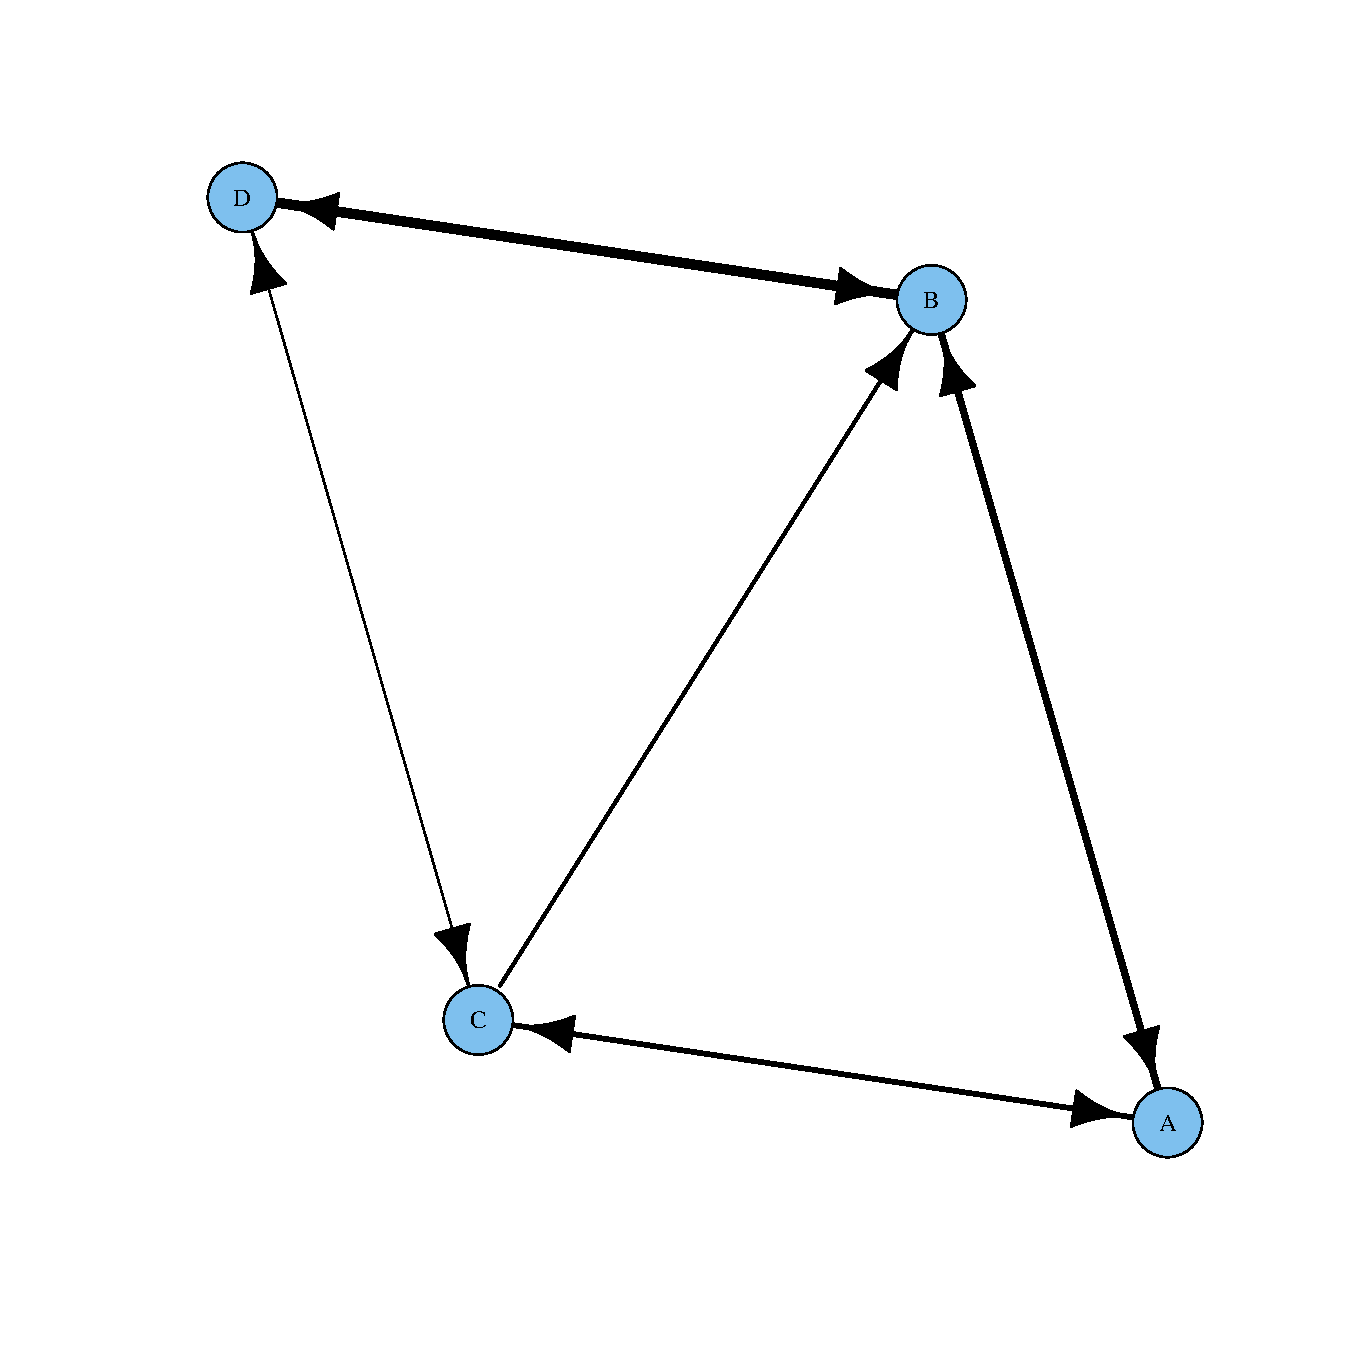
\includegraphics[width=7cm]{fig/metode/moneca_eksempel1.pdf}
}
\parbox[H]{8cm}{\null
\centering
  % \vskip-\abovecaptionskip
  \captionof{table}[t]{Adjacency matrice til netværk}%
  \vskip\abovecaptionskip
\begin{tabular}{@{}c|c|c|c|c@{}}
\multicolumn{1}{l|}{} & A & B & C & D \\ \midrule
A                     & - & - & - & - \\ \midrule
B                     & 4 & - & - & - \\ \midrule
C                     & 3 & 2 & - & - \\ \midrule
D                     & 0 & 6 & 1 & -
\end{tabular}
}
\end{figure}
%
Moneca ville i dette tilfælde komme frem til at netværket i figur \ref{monecaeksempel1} består af klyngerne [A|C] og [B|D]. Det sker ud fra følgende procedure: 
%
\begin{enumerate} \label{metode_monecastepbystep}
  \item Først lægges de to kraftigst forbundne noder sammen. Det vil her sige [B|D], hvor styrken af forbindelsen er seks.
  \item Derefter gør det den samme med de to næstmest forbundne noder, [A|B], der har en styrke på 4. Eftersom [B] allerede er en del af den foreløbige klynge [B|D], spørger Moneca om det er muligt at indlemme [A] i den allerede etablerede foreløbige klynge. Det kan ikke lade sig gøre, da [A|B] ikke er forbundne.
  \item Moneca går derfor videre til den tredje stærkeste forbindelse, [A|C]. Hverken [A] eller [C] er en del af en foreløbig klynge, og de lægges derfor sammen.
  \item Den fjerde stærkeste forbindelse er [B|C]. [B] og [C] er allerede parret med henholds [D] og [A], og Moneca beregner derfor om [A|B|C|D] udgør en klike, altså alle er forbundne med hinanden. Da det ikke er tilfældet, stopper Moneca og har dermed etableret klyngerne [A|C] og [B|D].
\end{enumerate}
% lidt usikker på om nedenstående bør tages med - det er jo beskrevet heroppe. Måske dobbeltkonfekt. 
Det vil sige at Moneca ikke etablerer nogen af de maksimale kliker, [A|B|C] eller [B|C|D]. Den semistrenge stopregel om klike-tilhørsforhold indenfor klynger betyder desuden, at man med en vis sindsro kan sige at en klynge rent faktisk \emph{er} en samlet størrelse - da den kun kan dannes hvis alle noderne har forbindelse til hinanden, hvilket eksemplet illustrerer: De to maksimale kliker etableres netop ikke, og hvis de gjorde, ville troværdigheden af grænsedragningen mellem klyngerne være langt mere tvivlsom.

For at opsummere ovenstående i mere generelle termer: Moneca starter med at slå noderne med de to mest intense forbindelser sammen til en foreløbig klynge, og går derefter videre til den næstmest intense forbindelse. Hvis en eller begge af noderne i de efterfølgende forbindelser allerede har forbindelse til en tredje eller fjerde node, vurderer Moneca, om denne indgår i en klike med den allerede etablerede klynge. Det er her vigtigt at understrege, at denne vurdering ikke er baseret på styrken af forbindelserne, men udelukkende om der eksisterer en forbindelse%
%
\footnote{Man kan forestille sig en fremtidig version af Moneca foretage en mere avanceret vurdering i disse tvivlsspørgsmål, hvori styrken af relationen kunne indgå som vurderingsgrundlag.}
%
. Moneca fortsætter med denne procedure i prioriteret rækkefølge fra de mest intense forbindelser til de mindst intense, indtil alle noder er placeret i kliker med andre noder, der endnu ikke er “optaget” af en mere intens forbindelse. Kriteriet for, om Moneca tillader at slå de tre noder sammen, er om de tilsammen former en klike, altså alle er forbundet til hinanden. Hvis de ikke er det, går den videre til den den næstmest intense forbindelse, og fortsætter med at forbinde noder indtil der ikke længere kan etableres flere kliker. Kriteriet om at allerede-etablerede klynger kun kan lægges sammen med nye noder, hvis disse indgår i en klike med alle medlemmer af klyngen, er den stop-regel, der gør at Moneca ikke bare ender med at etablere det redundante stykke information, at hvert enkelt komponent%
%
\footnote{Et komponent betyder en subgraf, hvor alle noder er forbundne gennem stier. Et netværk kan således bestå af flere komponenter, der per definition ikke er forbundne (ellers ville de være en del af samme komponent), samt noder uden forbindelse til andre noder (\emph{isolates}) \parencite[100]{Scott2000}.}% 
er en klynge i sig selv \parencite[8]{Touboel2015}. 

Efter denne  første segmentering er Moneca beregnet til at gentage proceduren indtil det ikke længere er muligt at skabe større segmenter, fordi den føromtalte klike-regel forhindrer det. Det er vigtigt at fremhæve, at Moneca i de efterfølgende klyngeinddelinger baseret den på side \pageref{monecastepbystep} beskrevne procedure, \emph{ikke} længere tager de oprindelige, interne forbindelser mellem grundkategorierne i betragtning, hvis disse er blevet lagt sammen med andre grundkategorier. I den efterfølgende klyngeinddeling vil de interne forbindelser mellem noderne på et lavere niveau ikke indgå i beregningerne i forbindelserne mellem de nyskabte noder. Det vil sige at klike-reglen kun tager højde for forbindelser til noder \emph{på det niveau noderne befinder sig på, og ikke forbindelserne på de lavere niveauer}. Når man vurderer kvaliteten af klyngerne på de højere niveauer, er det derfor centralt at se på en række standardmål for klyngens interne forbindelser, for at vurdere rimeligheden af at vurdere klyngen som en samlet størrelse. Det er dette spørgsmål vi nu afslutter gennemgangen af Moneca med.



% en lang række fordele ved at have fuld population i netværk, udover det argument vi brugte i adelsbogen, så også fx beregning af densitet (scott s. 74-5) mm. 



%%%%%%%%%%%%%%%%%%%%%%%%%%%%%%%%%%%%%%%%%%%%%%%%%%%%%%%%%%%
\subsection{Opsummering \label{}}
%%%%%%%%%%%%%%%%%%%%%%%%%%%%%%%%%%%%%%%%%%%%%%%%%%%%%%%%%%%


%%%%%%%%%%%%%%%%%%%%%%%%%%%%%%%%%%%%%%%%%%%%%%%%%%%%%%%%%%%
% Trash
%%%%%%%%%%%%%%%%%%%%%%%%%%%%%%%%%%%%%%%%%%%%%%%%%%%%%%%%%%%


%%%%%%%%%%%%%%%%%%%%%%%%%%%%%%%%%%%%%%%%%%%%%%%%%%%%%%%%%%%

%Local Variables: 
%mode: latex
%TeX-master: "report"
%End: